\section{Impact of Uneven Distribution\\ of Student Characteristics} % This title needs to be improved... [snarky comment from ANR to herself]

\begin{figure}[t]
    \centering
    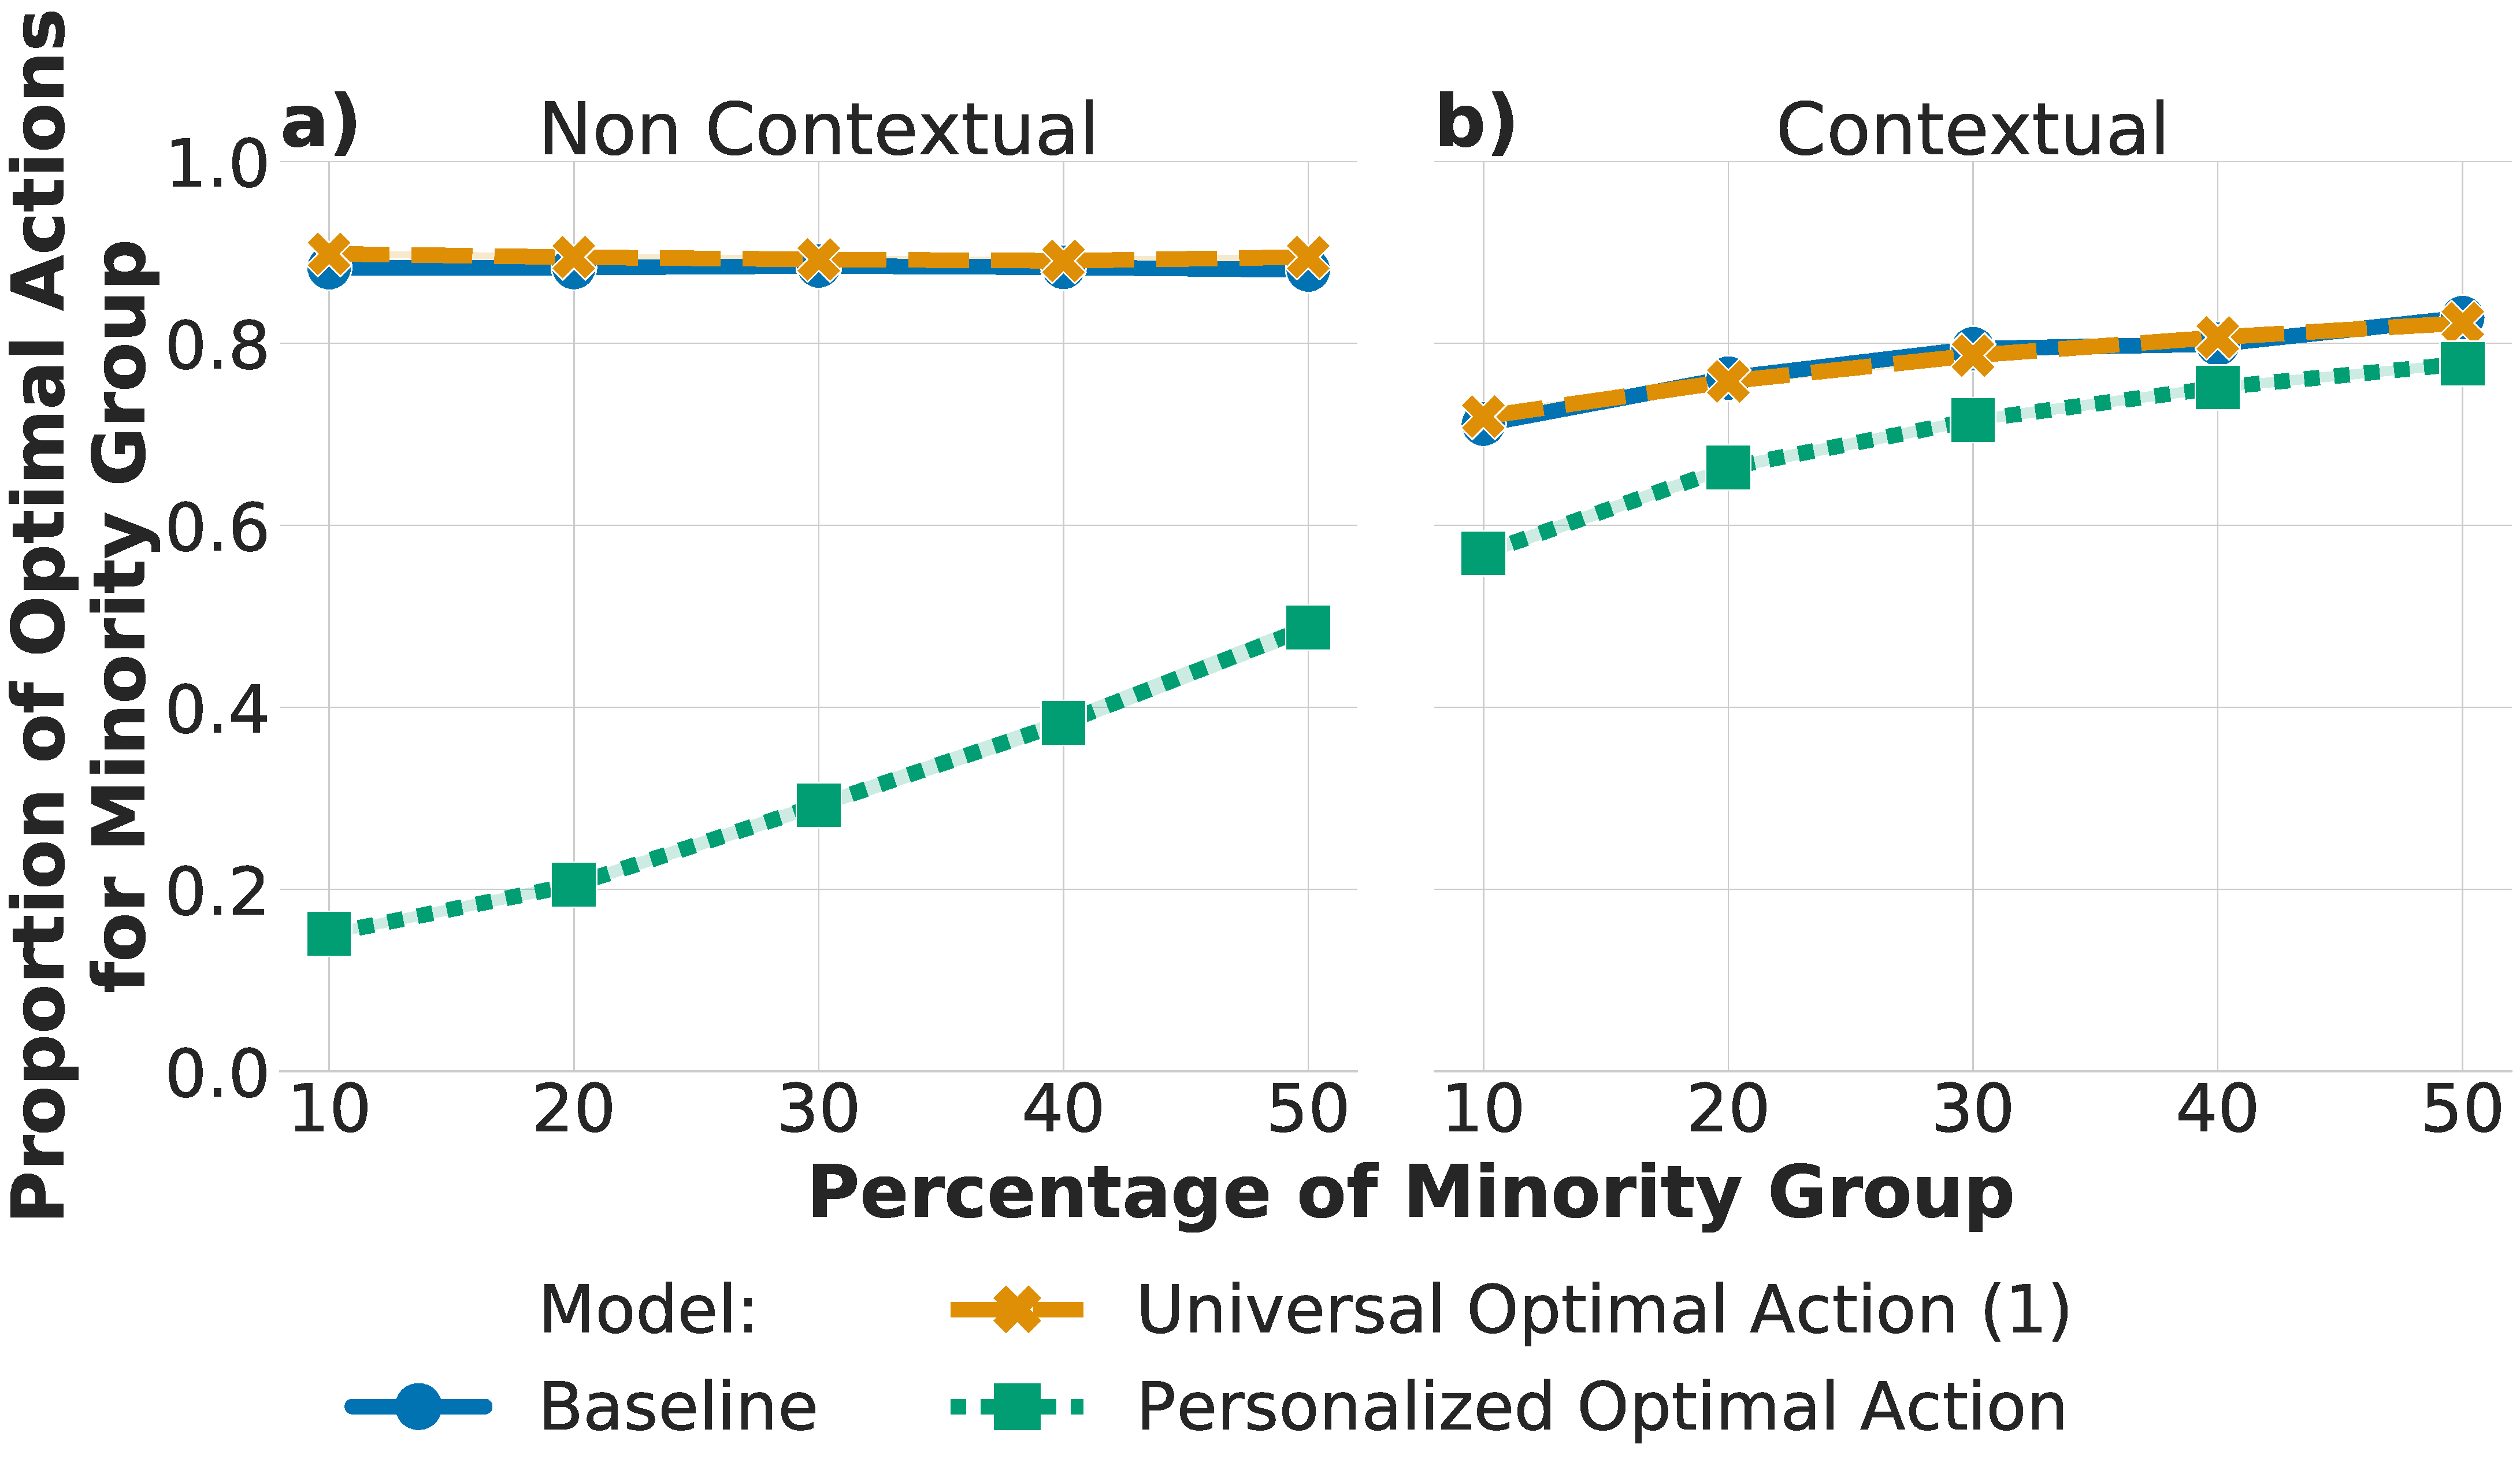
\includegraphics[width=\columnwidth]{figs/MinGrpSize.pdf}
    \caption{Proportion of optimal actions for minority groups with sizes of 10\%--50\% for the two bandit types across the three outcome-generating models, limited to one contextual variable. Standard errors, represented by the translucent bands, are negligible.}
    \label{fig:MinGrpSize1ConVar}
\end{figure}


The results of the previous simulations demonstrate that in situations where student characteristics (features) impact the outcome of different educational interventions, a contextual MAB algorithm only provides an improvement over a non-contextual algorithm when knowledge about the characteristic is necessary for choosing the best action. These simulations provided insight into how performance is impacted by different patterns of relationships between student characteristics and outcomes, with the assumption that those characteristics were uniformly distributed. However, in reality, some characteristics are likely to be more common than others. For example, when optimizing which hint to give to students who answer a question incorrectly, the algorithm is more likely to encounter a student with lower prior knowledge than one with higher prior knowledge.
% imagine a system that is choosing what intervention to give students who answer an exam question incorrectly. It is plausible that the most effective intervention is based on students' prior homework scores, but of students who answer incorrectly, more will tend to have low prior scores than high scores. 
Thus we now relax this assumption and explore how changing the distribution of student characteristics impacts student outcomes for both types of MAB algorithms. In these simulations, we examined not only overall outcomes, but also outcomes for different groups of students. Attention to group-specific outcomes is vital for identifying inequitable impacts of adaptive algorithms. %need to strengthen this point a bit


\subsection{Methods}

Similar to the first set of simulations, we compared non-contextual and contextual MAB implementations that used Thompson sampling across the same three horizons of 50, 250, and 1000 students, with a focus on 250; we repeated each simulation 1000 times. These simulations include a new independent variable: the proportion of students in each group. Specifically, for each simulated student, we varied the probability of the student being in the minority group (i.e., having a value of one for the first student characteristic) from 10\% to 50\%, using 10\% increments. 
% In our analyses of results, we group students into a minority group, which has the smaller probability of being enacted, and a majority group. At 50\%, the minority and majority groups have equal expected size.
In addition to analyzing performance across all students, we examined performance for both the minority and majority groups separately. We also examined the \textit{balanced success rate}, defined as the simple average of the group-specific performances~\cite{ben2010user}. Balanced success rate provides a way of examining performance that treats each group as equally important, even though one group may have more students than another.

\begin{figure*}[t]
    \centering
    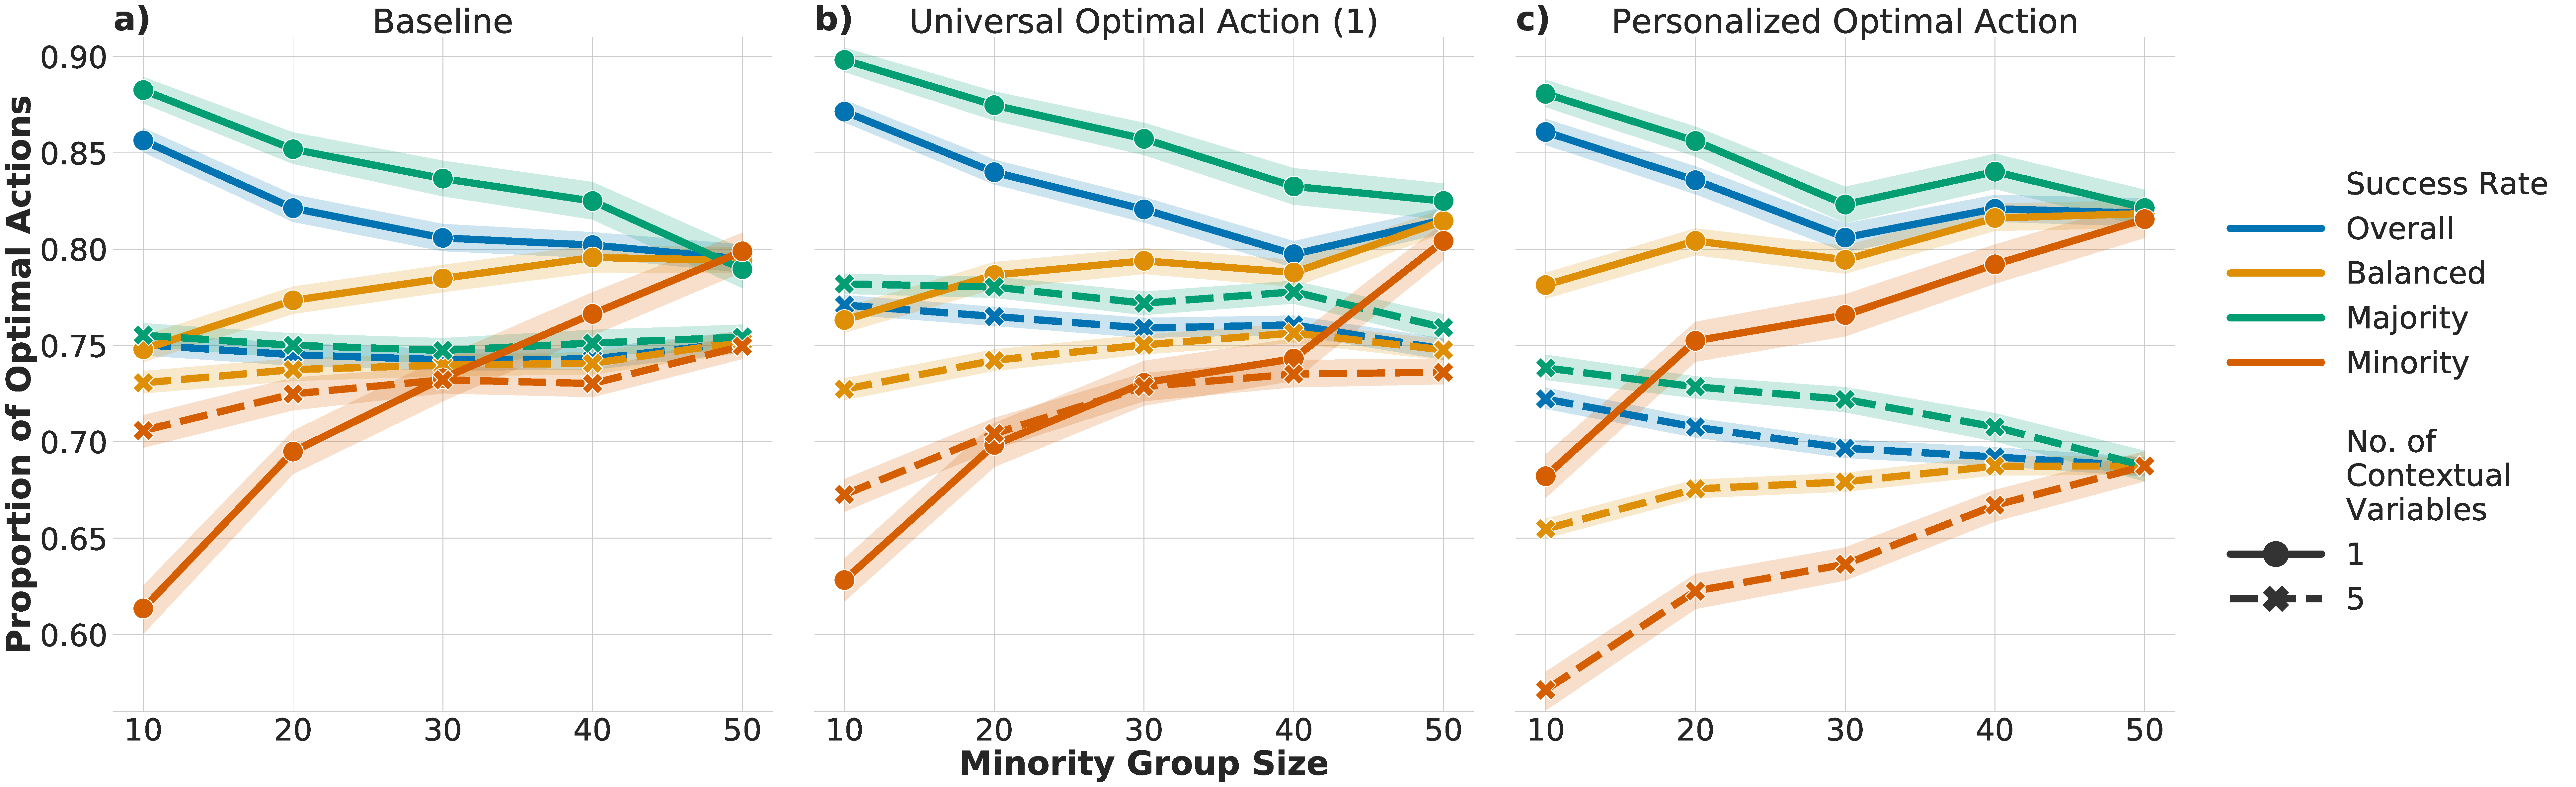
\includegraphics[width=\textwidth]{figs/MinGrpSize1v5.pdf}
    \caption{Comparing the proportion of optimal actions of the contextual bandit between 1 and 5 student features (i.e., contextual variables) for the majority and minority groups, as well as their balanced and overall averages, across minority group sizes of 10\%--50\%. Standard errors, represented by the translucent bands, are negligible.}
    \label{fig:Balanced_Success_Graph}
\end{figure*}
 
\subsection{Results}



% \begin{itemize}
%     \item First start with if we just have one contextual variable, what happens.
%     \item Then include something showing for one of the minority group sizes (20 or 30\%), what happens as the number of contextual variables increases.
%     \item Include some ANOVAs here to make sense of things.
% \end{itemize}


As in the previous analysis, we used an ANCOVA to compare the performance for the two bandit types in terms of the proportion of optimal actions, but this time treating the percentage of the minority group as a covariate. 

% Similar to the previous analysis, we focused on analyzing the performance of the two MAB algorithms for the three types of outcome-generating models for 250 students across 1000 trials. To compare the proportion of optimal actions across the two bandit types, we again used an ANCOVA, treating the percentage of the minority group as a covariate. 
%An analysis of covariance (ANCOVA) was used to examine the difference in performance between the two bandit types, in terms of proportion of optimal actions, while controlling for the percentage of the minority group.

\textbf{One student characteristic:} With one student characteristic, the contextual MAB algorithm's performance for the minority group decreases as the size of the minority group becomes smaller, across all outcome-generating models (Figure~\ref{fig:MinGrpSize1ConVar}b and Figure~\ref{fig:Balanced_Success_Graph}; $t(59996)=-33.962$, $p<0.001$, $b=-0.427$, 95\% CI = $[-0.452, -0.402]$).
This leads the contextual MAB algorithm to have a lower balanced success rate for smaller minority groups. However, overall performance across all students is slightly better since so many more students are in the majority group (Figure~\ref{fig:Balanced_Success_Graph}; $t(59996)=16.633$, $p<0.001$, $b=0.126$, 95\% CI = $[0.111, 0.141]$). In other words, decreasing the minority group size hurts the minority group more than it helps the majority group on a per-student basis; but replacing students from the minority group, who are assigned worse conditions, with students from the majority group, who are assigned better conditions, increases overall reward.  

This pattern of results occurs because the contextual MAB has more uncertainty about the impact of the particular value of the student characteristic that appeared fewer times: in the least balanced case, we expect the minority group to be seen only 25 times on average given a horizon of 250 students. Hence, providing a model with the potential to personalize for a minority group is a calculated risk - although the extra expressivity is likely intended to improve experiences for all groups of students, it can negatively impact minority groups, with a larger negative impact for smaller minority groups.

In contrast, the non-contextual MAB algorithm is relatively unaffected by the changing distribution of student characteristics in both the baseline ($t(9996)=0.497$, $p=0.619$) and universal optimal action scenarios ($t(39996)=1.506$, $p=0.132$), as shown by Figure~\ref{fig:MinGrpSize1ConVar}a. The changing distribution of student characteristics changes the expected rate of obtained reward from each action, but the changes are small enough that they have little impact on the algorithm's ability to choose optimal actions.
% This is perhaps surprising in the latter case because as the distribution of students changes, the amount of variance in each condition is also changed. For example, in one of the four group independent policy cases, a student in the minority group has a positive outcome 80\% of the time with action 1 and 90\% of the time with action 2, compared to 40\% and 60\% for a student in the majority group. There is a slight trend in this case for lowered performance given a moderate amount of students in the minority group, with the poorest performance occurring with 30\% of students in the minority group, but the overall difference in performance is slight. 

However, for the personalized optimal action model, the size of the minority group \textit{does} have a large impact on individual student outcomes for the non-contextual MAB algorithm: when the minority group is small, the algorithm learns to choose the action that is best for the majority and worst for the minority, resulting in the optimal action being chosen only 15\% of the time for the minority group, within a horizon of 250 students (Figure~\ref{fig:MinGrpSize1ConVar}a). When the two groups are of equal size, the algorithm has no systematic information that shows one action as consistently better or worse than the other; thus on average, it chooses the optimal action about 50\% of the time for both groups. 


\textbf{Additional student characteristics for the contextual MAB algorithm:} When the number of student characteristics increases, the impact on the minority and majority groups differs for the baseline and universal optimal action models compared to the personalized optimal action  (Figure~\ref{fig:Balanced_Success_Graph}). In the two former models, the impact on balanced success rate is generally small: as the number of student characteristics increases from one to five, balanced success decreases no more than 8\%, except by 11\% in universal optimal action (4); for most of these models, the decrease is even smaller when the minority group is smaller.
In these models, the algorithm's performance for small minority groups is improved with more student characteristics, while performance for majority groups decreases. For example, in the baseline scenario with 10\% of students in the minority group, the algorithm chooses the optimal action for 71\% of the minority group when there are five student characteristics, compared to 61\% of these students when there is only one student characteristic.
More student characteristics leads to more exploration with the initial students, and thus the algorithm is less likely to systematically execute a bad policy for the minority group based on a small number of initial samples. 

% balanced success rate for the contextual MAB algorithm decreases, regardless of the size of the minority group or outcome-generating scenario.
% The pattern of results that generates this lowered success rate 
% Increasing the number of contextual variables tends to hurt the majority group, while helping the mino
% However, the difference in balanced success rates is largest when the two groups are of equal size, and with the exception of the personalized optimal action scenario, the difference in balanced success rates tends to be smaller when the minority group is smaller. 
% This results from the fact that, again with the exception of the personalized optimal action scenario, the algorithm's performance for small minority groups is actually better with more contextual variables. For example, in the baseline scenario with 10\% of students in the minority group, the algorithm chooses the optimal action for 71\% of the 250 students when there are five contextual variables, compared to 61\% of the students when there is only one contextual variable. This occurs because more contextual variables leads to more exploration with the initial students, and thus the algorithm is less likely to systematically execute a suboptimal policy for the minority group due to drawing conclusions from a small number of initial samples. 

For the personalized optimal action scenario, increasing the number of student characteristics from one to five decreases performance for both minority and majority groups by about 15\% regardless of the size of the minority group, uniformly lowering balanced success rate. Due to the extra exploration caused by the extraneous student characteristics, the algorithm is slower to exploit the actual relationship between the relevant student characteristic and the action choice, without differential impact based on minority group size.
%, combined with fewer students from which to learn about the minority group, means that the extra exploration that improves performance in the other scenarios hurts performance in this case: the algorithm is less quick to exploit the actual relationship between the relevant student characteristic and the action choice.

% Key patterns:
% \begin{itemize}
%     \item When minority group is small, there's improved performance *for the minority group* with 5 variables for most scenarios. Reason: more exploration early on, less likely to systematically fall into a suboptimal policy for any particular group.
%     \item But as minority group size grows, performance changes less quickly with 5 CVs: more exploration still happening at the same horizon, because less confident in conclusions.
%     \item For the case where the policy does depend on the CV, there's decreased performance for the minority group for all of the minority group sizes when there are 5 CVs. That's because the extra CVs make it harder to find a true interaction when there is one.
%     \item BSR: Lower for CV = 5 as expected. Appears that as minority group size increases, for all but crossover the difference in performance increases slightly. For crossover, size of effect is relatively constant.
% \end{itemize}

\iffalse % block comment


\begin{table*}
\caption{Proportion optimal actions, horizon = 250, all group sizes, performance across all groups and CV = 1.}
\begin{tabular}{lrrrrr}
\toprule
Minority Group Size &        10 &        20 &        30 &        40 &        50 \\
Bandit and Effect Type      &           &           &           &           &           \\
\midrule
ModContextual,None      &  0.856348 &  0.821244 &  0.805808 &  0.802108 &  0.794872 \\
ModContextual,Main (1)      &  0.871400 &  0.839916 &  0.820596 &  0.797332 &  0.815184 \\
ModContextual,Interaction48 &  0.933624 &  0.907804 &  0.887108 &  0.866224 &  0.854288 \\
ModContextual,Interaction57 &  0.855780 &  0.820044 &  0.804564 &  0.804548 &  0.793884 \\
ModContextual,Interaction89 &  0.790200 &  0.790876 &  0.764876 &  0.781476 &  0.784140 \\
ModContextual,Crossover &  0.860764 &  0.835756 &  0.805980 &  0.820940 &  0.818588 \\
NonContextual,None      &  0.891668 &  0.877504 &  0.883992 &  0.883216 &  0.884636 \\
NonContextual,Main (1)      &  0.899700 &  0.899288 &  0.897256 &  0.884064 &  0.892628 \\
NonContextual,Interaction48 &  0.959292 &  0.957744 &  0.949364 &  0.944288 &  0.935956 \\
NonContextual,Interaction57 &  0.890644 &  0.883288 &  0.890980 &  0.887544 &  0.888996 \\
NonContextual,Interaction89 &  0.838168 &  0.826292 &  0.823028 &  0.841332 &  0.849556 \\
NonContextual,Crossover &  0.776756 &  0.670608 &  0.580048 &  0.521512 &  0.501544 \\
\bottomrule
\end{tabular}
\end{table*}

\begin{table*}
\caption{Proportion optimal actions, horizon = 250, all group sizes, performance for group 0 and CV = 1.}
\begin{tabular}{lrrrrr}
\toprule
Minority Group Size &        10 &        20 &        30 &        40 &        50 \\
Bandit and Effect Type      &           &           &           &           &           \\
\midrule
ModContextual,None      &  0.613523 &  0.694961 &  0.732960 &  0.766390 &  0.798822 \\
ModContextual,Main (1)     &  0.628272 &  0.698429 &  0.730649 &  0.743170 &  0.804242 \\
ModContextual,Interaction48 &  0.595183 &  0.702625 &  0.730411 &  0.750989 &  0.782653 \\
ModContextual,Interaction57 &  0.622903 &  0.678792 &  0.717704 &  0.779673 &  0.796462 \\
ModContextual,Interaction89 &  0.598684 &  0.678936 &  0.743387 &  0.774596 &  0.823764 \\
ModContextual,Crossover &  0.682151 &  0.752437 &  0.765803 &  0.792061 &  0.815562 \\
NonContextual,None      &  0.893786 &  0.876132 &  0.883945 &  0.884595 &  0.883612 \\
NonContextual,Main (1)     &  0.901123 &  0.898164 &  0.898399 &  0.883778 &  0.892063 \\
NonContextual,Interaction48 &  0.958717 &  0.957539 &  0.949884 &  0.944494 &  0.936221 \\
NonContextual,Interaction57 &  0.891941 &  0.884045 &  0.890403 &  0.887577 &  0.890546 \\
NonContextual,Interaction89 &  0.836723 &  0.828386 &  0.823892 &  0.841261 &  0.849212 \\
NonContextual,Crossover &  0.149687 &  0.213161 &  0.294141 &  0.379826 &  0.484818 \\
\bottomrule
\end{tabular}
\end{table*}

\begin{table*}
\caption{Balanced success rate for proportion optimal actions - horizon = 250, 1 CV}
\begin{tabular}{lrrrrr}					
\toprule					
Minority Group Size &        10 &        20 &        30 &        40 &        50 \\					
Bandit and Effect Type - BSR  &           &           &           &           &           \\					
\midrule					
ModContextual,None      	   &    0.748016	& 0.773401	& 0.7847735	& 0.795648	& 0.794208      \\
ModContextual,Main      	   &    0.7632115	& 0.7865455	& 0.793931	& 0.78784	  & 0.8145985     \\
ModContextual,Interaction48  &    0.7831475	& 0.8307925	& 0.842807	& 0.8463	  & 0.8539765     \\
ModContextual,Interaction57  &    0.7521865	& 0.7665245	& 0.7793055	& 0.79957	  & 0.793037      \\
ModContextual,Interaction89  &    0.7045975	& 0.748741	& 0.7585305	& 0.779965	& 0.783931      \\
ModContextual,Crossover 	   &    0.7813535	& 0.8042625	& 0.794461	& 0.8161455	& 0.8184485     \\
NonContextual,None      	   &    0.8926215	& 0.8769845	& 0.883969	& 0.8834765	& 0.884669      \\
NonContextual,Main      	   &    0.900343	& 0.898902	& 0.897586	& 0.884048	& 0.892659      \\
NonContextual,Interaction48  &    0.959022	& 0.957682	& 0.9494705	& 0.944336	& 0.9359175     \\
NonContextual,Interaction57  &    0.891247	& 0.883549	& 0.8908255	& 0.8875825	& 0.88897       \\
NonContextual,Interaction89  &    0.837544	& 0.8271395	& 0.8232795	& 0.8413645	& 0.849524      \\
NonContextual,Crossover 	   &    0.49779 	& 0.4982355	& 0.497484	& 0.496847	& 0.4987915     \\
\bottomrule					
\end{tabular}
\end{table*}

\begin{table*}
\caption{Proportion optimal actions, horizon = 250, all group sizes, performance for group 1 and CV = 1.}

\begin{tabular}{lrrrrr}
\toprule
Minority Group Size &        10 &        20 &        30 &        40 &        50 \\
Bandit and Effect Type  &           &           &           &           &           \\
\midrule
ModContextual,None      &  0.882509 &  0.851841 &  0.836587 &  0.824906 &  0.789594 \\
ModContextual,Main      &  0.898151 &  0.874662 &  0.857213 &  0.832510 &  0.824955 \\
ModContextual,Interaction48 &  0.971112 &  0.958960 &  0.955203 &  0.941611 &  0.925300 \\
ModContextual,Interaction57 &  0.881470 &  0.854257 &  0.840907 &  0.819467 &  0.789612 \\
ModContextual,Interaction89 &  0.810511 &  0.818546 &  0.773674 &  0.785334 &  0.744098 \\
ModContextual,Crossover &  0.880556 &  0.856088 &  0.823119 &  0.840230 &  0.821335 \\
NonContextual,None      &  0.891457 &  0.877837 &  0.883993 &  0.882358 &  0.885726 \\
NonContextual,Main      &  0.899563 &  0.899640 &  0.896773 &  0.884318 &  0.893255 \\
NonContextual,Interaction48 &  0.959327 &  0.957825 &  0.949057 &  0.944178 &  0.935614 \\
NonContextual,Interaction57 &  0.890553 &  0.883053 &  0.891248 &  0.887588 &  0.887394 \\
NonContextual,Interaction89 &  0.838365 &  0.825893 &  0.822667 &  0.841468 &  0.849836 \\
NonContextual,Crossover &  0.845893 &  0.783310 &  0.700827 &  0.613868 &  0.512765 \\
\bottomrule
\end{tabular}
\end{table*}

\fi

